\let\negmedspace\undefined{}
\let\negthickspace\undefined{}
\documentclass[journal,12pt,twocolumn]{IEEEtran}
 \usepackage{gensymb}
 \usepackage{polynom}
\usepackage{amssymb}
\usepackage[cmex10]{amsmath}
\usepackage{amsthm}
 \usepackage{stfloats}
\usepackage{bm}
 \usepackage{longtable}
 \usepackage{enumitem}
 \usepackage{mathtools}
 \usepackage{tikz}
 \usepackage[breaklinks=true]{hyperref}
\usepackage{listings}
\usepackage{color}                                            
\usepackage{array}                                            
\usepackage{longtable}                                        
\usepackage{calc}                                             
    \usepackage{multirow}                                         
    \usepackage{hhline}                                           
    \usepackage{ifthen}                                           
    \usepackage{lscape}     
\DeclareMathOperator*{\Res}{Res}
\DeclareMathOperator*{\equals}{=}
\renewcommand\thesection{\arabic{section}}
\renewcommand\thesubsection{\thesection.\arabic{subsection}}
\renewcommand\thesubsubsection{\thesubsection.\arabic{subsubsection}}
\renewcommand\thesectiondis{\arabic{section}}
\renewcommand\thesubsectiondis{\thesectiondis.\arabic{subsection}}
\renewcommand\thesubsubsectiondis{\thesubsectiondis.\arabic{subsubsection}}
\hyphenation{op-tical net-works semi-conduc-tor}
\def\inputGnumericTable{}                                 %%
\lstset{
frame=single, 
breaklines=true,
columns=fullflexible
}
\begin{document}
\newtheorem{theorem}{Theorem}[section]
\newtheorem{problem}{Problem}
\newtheorem{proposition}{Proposition}[section]
\newtheorem{lemma}{Lemma}[section]
\newtheorem{corollary}[theorem]{Corollary}
\newtheorem{example}{Example}[section]
\newtheorem{definition}[problem]{Definition}
\newcommand{\BEQA}{\begin{eqnarray}}
\newcommand{\EEQA}{\end{eqnarray}}
\newcommand{\define}{\stackrel{\triangle}{=}}
\newcommand*\circled[1]{\tikz[baseline= (char.base)]{
    \node[shape=circle,draw,inner sep=2pt] (char) {#1};}}
\bibliographystyle{IEEEtran}
\providecommand{\mbf}{\mathbf}
\providecommand{\pr}[1]{\ensuremath{\Pr\left(#1\right)}}
\providecommand{\qfunc}[1]{\ensuremath{Q\left(#1\right)}}
\providecommand{\sbrak}[1]{\ensuremath{{}\left[#1\right]}}
\providecommand{\lsbrak}[1]{\ensuremath{{}\left[#1\right.]}}
\providecommand{\rsbrak}[1]{\ensuremath{{}\left[#1\right.]}}
\providecommand{\brak}[1]{\ensuremath{\left(#1\right)}}
\providecommand{\lbrak}[1]{\ensuremath{\left(#1\right.)}
\providecommand{\rbrak}[1]{\ensuremath{\left[#1\right.]}}}
\providecommand{\cbrak}[1]{\ensuremath{\left\{#1\right\}}}
\providecommand{\lcbrak}[1]{\ensuremath{\left\{#1\right.}}
\providecommand{\rcbrak}[1]{\ensuremath{\left.#1\right\}}}
\theoremstyle{remark}
\newtheorem{rem}{Remark}
\newcommand{\sgn}{\mathop{\mathrm{sgn}}}
\providecommand{\abs}[1]{\left\vert#1\right\vert}
\providecommand{\res}[1]{\Res\displaylimits_{#1}} 
\providecommand{\norm}[1]{\left\lVert#1\right\rVert}
\providecommand{\mtx}[1]{\mathbf{#1}}
\providecommand{\mean}[1]{E\left[ #1 \right]}
\providecommand{\fourier}{\overset{\mathcal{F}}{ \rightleftharpoons}}
\providecommand{\system}{\overset{\mathcal{H}}{ \longleftrightarrow}}
\newcommand{\solution}{\noindent \textbf{Solution: }}
\newcommand{\cosec}{\,\text{cosec}\,}
\newcommand*{\permcomb}[4][0mu]{{{}^{#3}\mkern#1#2_{#4}}}
\newcommand*{\perm}[1][-3mu]{\permcomb[#1]{P}}
\newcommand*{\comb}[1][-1mu]{\permcomb[#1]{C}}
\renewcommand{\thetable}{\arabic{table}} 
\providecommand{\dec}[2]{\ensuremath{\overset{#1}{\underset{#2}{\gtrless}}}}
\newcommand{\myvec}[1]{\ensuremath{\begin{pmatrix}#1\end{pmatrix}}}
\newcommand{\mydet}[1]{\ensuremath{\begin{vmatrix}#1\end{vmatrix}}}
\numberwithin{equation}{section}
\numberwithin{figure}{section}
\numberwithin{table}{section}
\makeatletter
\@addtoreset{figure}{problem}
\makeatother
\let\StandardTheFigure\thefigure{}
\let\vec\mathbf{}
%\renewcommand{\thefigure}{\theproblem}
\def\putbox#1#2#3{\makebox[0in][l]{\makebox[#1][l]{}\raisebox{\baselineskip}[0in][0in]{\raisebox{#2}[0in][0in]{#3}}}}
     \def\rightbox#1{\makebox[0in][r]{#1}}
     \def\centbox#1{\makebox[0in]{#1}}
     \def\topbox#1{\raisebox{-\baselineskip}[0in][0in]{#1}}
     \def\midbox#1{\raisebox{-0.5\baselineskip}[0in][0in]{#1}}
\vspace{3cm}
\title{Assignment:Random Variables }
\author{Pranav B (AI21BTECH11023)}
\maketitle
\newpage
\bigskip
\renewcommand{\thefigure}{\theenumi}
\renewcommand{\thetable}{\theenumi}
	% The solution
	\section{Solution:}
(1.3)Since U is an uniform random variable distribution, $P_{U}(x_{i})=P_{U}(x_{j})=k$,$\forall i,j$\\
	CDF of $P_{U}(x)$=$F_{U}(x)$\\
	\begin{align}
	=\int P_{U}(x) dx\\
	=\int k dx\\
  \text{wkt} \int_{0}^{1} kdx=1\\
  \therefore k=1\\
  \therefore F_{U}(x)=x
	\end{align}	
		\begin{figure}[h]
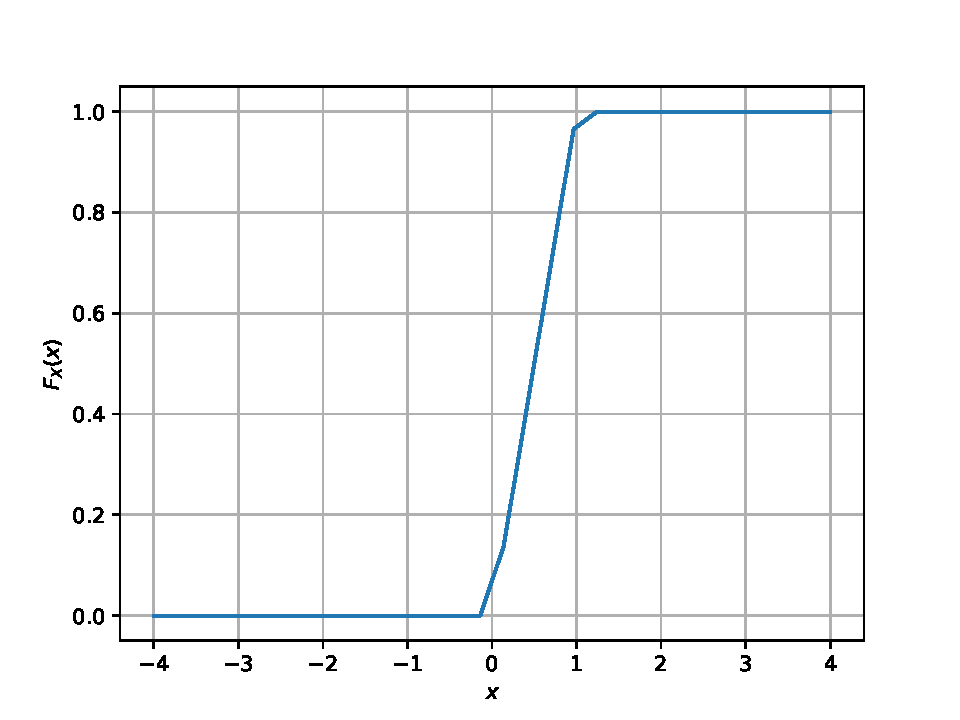
\includegraphics[width=0.5\textwidth]{uni_cdf.pdf}
\caption{CDF for (1)}
\label{fig:my_label}
\end{figure}
\\
(1.5) $dF_{U}(x)=dx$
\begin{align}
&\therefore E[U^k]=\int_{-\infty}^{\infty} x^k dx\\
&E[U]=\int_{0}^{1} x dx=\frac{1}{2}\\
&E[U^2]=\int_{0}^{1} x^2 dx=\frac{1}{3}\\
&\because P_{X}(x)=0 ,\forall x \in (1,\infty)\cap (-\infty,0)\\
&Var(X)=E[U^2]-(E[U])^2=\frac{1}{3}-\frac{1}{4}=\frac{1}{12}
\end{align}
(2.3) \begin{itemize}
\item PDF is symmetric about $x=0$\\
\item graph is bell shaped\\
\item mean of graph is situated at the apex point of the bell\\
\end{itemize}
		\begin{figure}[h]
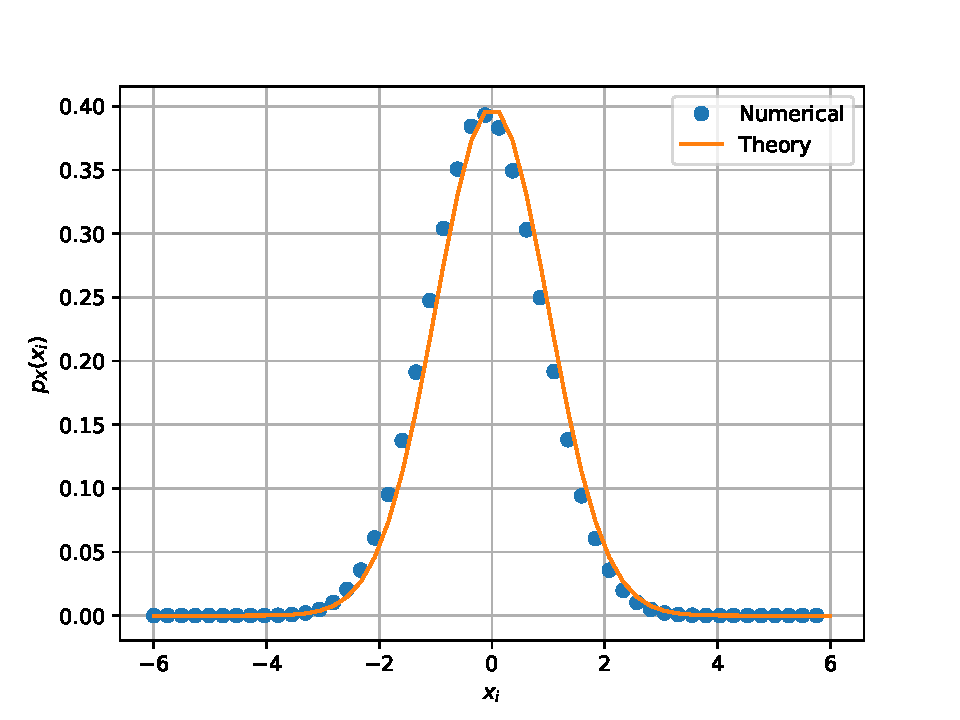
\includegraphics[width=0.5\textwidth]{gauss_pdf.pdf}
\caption{PDF for (2)}
\label{fig:my_label}
\end{figure}
(2.5) Given ,$p_{X}(x)=\frac{1}{\sqrt{2\pi}} e^{\frac{-x^2}{2}}$\\
 $F_{X}(x)=\int_{-\infty}^{x} p_{X}(x) dx$\\
 \begin{align}
  &=\int_{-\infty}^{x} \frac{1}{\sqrt{2\pi}} e^{\frac{-x^2}{2}} dx\\
 &=\frac{1}{2} erf\left(\frac{x}{\sqrt{2}}\right)\\
 &E[x]=\int_{-\infty}^{\infty} x p_{X}(x) dx\\
 &=\int_{-\infty}^{\infty} \frac{1}{\sqrt{2 \pi}} x e^{-\frac{-x^2}{2}}\\
  &\because x e^{-\frac{-x^2}{2}} \text{is a odd function},\\
  \nonumber
   &E[x]=0\\
 &E[x^2]=\int_{-\infty}^{\infty} x^2 p_{X}(x) dx\\
 &=\int_{-\infty}^{\infty} \frac{1}{\sqrt{2\pi}} x(xe^{-\frac{-x^2}{2}}) dx
 \end{align}
  Using integration by parts:
  \begin{align}
   \label{eq:eq1}
 & =x\int xe^{-\frac{-x^2}{2}} dx-\int\frac{d(x)}{dx} \int xe^{-\frac{-x^2}{2}}dx\\
 &I=\int x e^{-\frac{-x^2}{2}}\\
 &\text{Let} \frac{x^2}{2}=t \\
 &\implies x dx=dt\\
 &\implies =\int e^{-t} dt=-e^{-t} +c\\
 \label{eq:eq2}
 &\therefore \int x e^{-\frac{-x^2}{2}}=-e^{-\frac{-x^2}{2}} +c
 \end{align}
 Using \eqref{eq:eq2} in \eqref{eq:eq1}\\
 \begin{align}
&= -x e{-\frac{-x^2}{2}}+\int e^{-\frac{-x^2}{2}} dx\\
&\text{Also} ,\int_{-\infty}^{\infty} e^{-\frac{-x^2}{2}} dx=\sqrt{2 \pi} \\
&\therefore \text{substituting limits we get}, E[x^2]=1\\
 &Var(X)=E[x^2]-(E[x])^2=1-0
 \end{align}
 \begin{figure}[h]
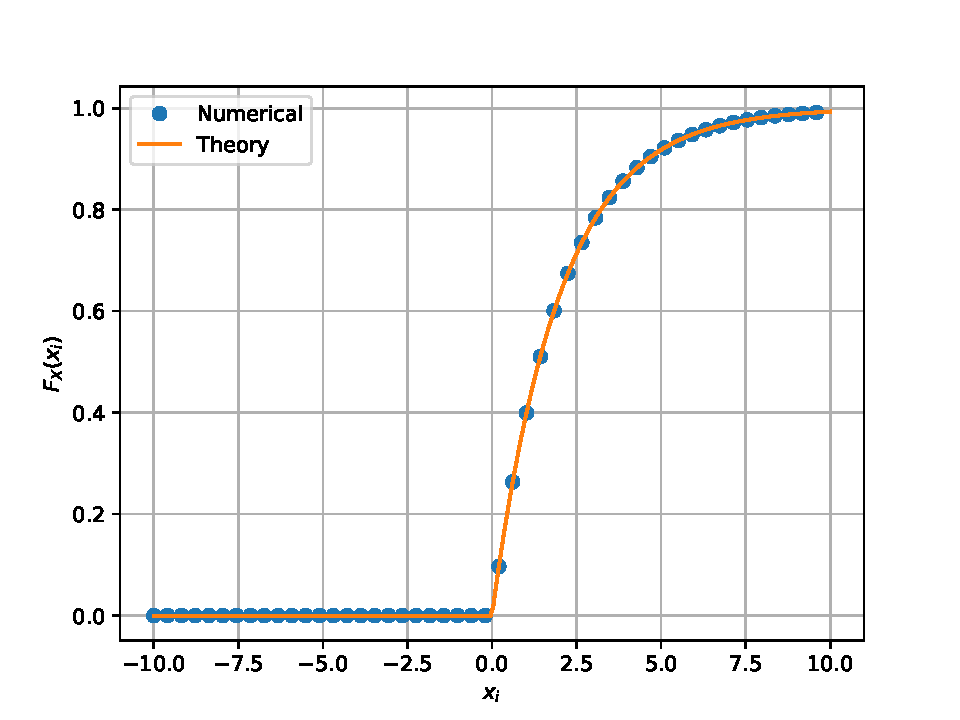
\includegraphics[width=0.5\textwidth]{V_cdf.pdf}
\caption{CDF for (3)}
\label{fig:my_label}
\end{figure}
\\
 (3.2)\begin{align}
 &F_{V}(x)=P(V \leq x)\\
 &=P(-2 ln(1-U) \leq x)\\
 &=P(1-e^{\frac{-x}{2}} \geq U)\\
 &P(U<x)=\int_{0}^{x} dx=x\\
 &\therefore P(1-e^{\frac{-x}{2}} \geq U)=1-e^{\frac{-x}{2}}, \forall x\geq 0 \\ 
 \nonumber
 \end{align}
\end{document}
